% supplementary_retention.tex
\subsection{Comparison-Data Misfit Profiles: Crisp Versus Graded Structure}

The comparison data method of \citet{ruscio-roche-2012} frames retention
as model comparison rather than null-hypothesis testing: for each
candidate count $k$, a finite population of comparison data with a known
$k$-factor structure is generated to reproduce the observed correlation
matrix and marginal distributions, bootstrap samples of the empirical
size are drawn from it, and the root-mean-square residual (RMSR) between
each sample's eigenvalue profile and the observed profile records how
well $k$ factors account for the full spectrum. Because each step
conditions on the structure already established, the method sidesteps
the choice of a structureless null that the main text identifies as the
weak point of the adapted parallel analysis. Comparison populations are
built by an iterative rank-remapping refinement after the GenData
algorithm of \citet{ruscio-kaczetow-2008}. \texttt{sfa\_cd()}
implements this profile for embedding similarity matrices, with
embedding dimensions in the case role: the Pearson correlations of the
transposed embedding matrix equal the \texttt{mean\_centered\_pearson}
similarity, so the profile addresses exactly the matrix the main
analyses factor. Profiles below use ten candidate counts, 500
bootstrap samples per count, populations of 10{,}000, and seed 42, for the three Qwen3-Embedding model sizes and
for a keyed random subsample of $n = \valCdHumanN$ respondents from the
human benchmark.

Figure~\ref{fig:cd-profiles} shows the result. The human responses
behave the way validated retention theory expects: relative improvement
climbs with each added factor and peaks at the fifth
(\valCdHumanImpFive\% improvement over four factors), after which it
collapses (\valCdHumanImpSix\% at the sixth), leaving
\valCdHumanNormFive{} of the one-factor misfit by $k = 5$. The
eigenvalue spectrum of real Big Five responses carries a crisp factor
boundary, and the profile finds it exactly where theory puts it. The
three embedding matrices show no such elbow: their profiles decline
smoothly (roughly \valCdEmbImpLow{} to \valCdEmbImpHigh{} percent relative
improvement per added factor, with no spike at any count), and
\valCdEmbNormFiveRange{} of the one-factor misfit remains at $k = 5$.
A factor model with diagonal uniqueness cannot reproduce the heavy
anisotropic tail of an embedding similarity spectrum, so every added
comparison factor keeps improving reproduction.

The sequential stopping rule of \citet{ruscio-roche-2012}, run at its
recommended liberal $\alpha = .30$ to document the point, saturates at
the ten-factor cap for all three embedding matrices. The human anchor
shows why this is a power phenomenon rather than an embedding
peculiarity: the rule terminates at \valCdCrossTwoFiftyWord{} factors only
toward the bottom of the method's validated sample-size range (250
respondents) and saturates to \valCdCrossSatWord{} from 500 respondents
up, mirroring the \valHumanPaKWord{} factors that conventional parallel
analysis suggests for the full benchmark ($n = \valNHuman$) in the main
text. On response data the test
eventually resolves real minor factors past the interpretable five; on
embedding matrices there is no boundary for it to find at all. Read
jointly, the profiles support the manuscript's practice of reporting
retention as a multi-criterion consensus with congruence tracked across
candidate counts, and its treatment of single-count verdicts on
embedding similarity matrices as depth choices rather than discoveries.

\begin{figure}[H]
\centering
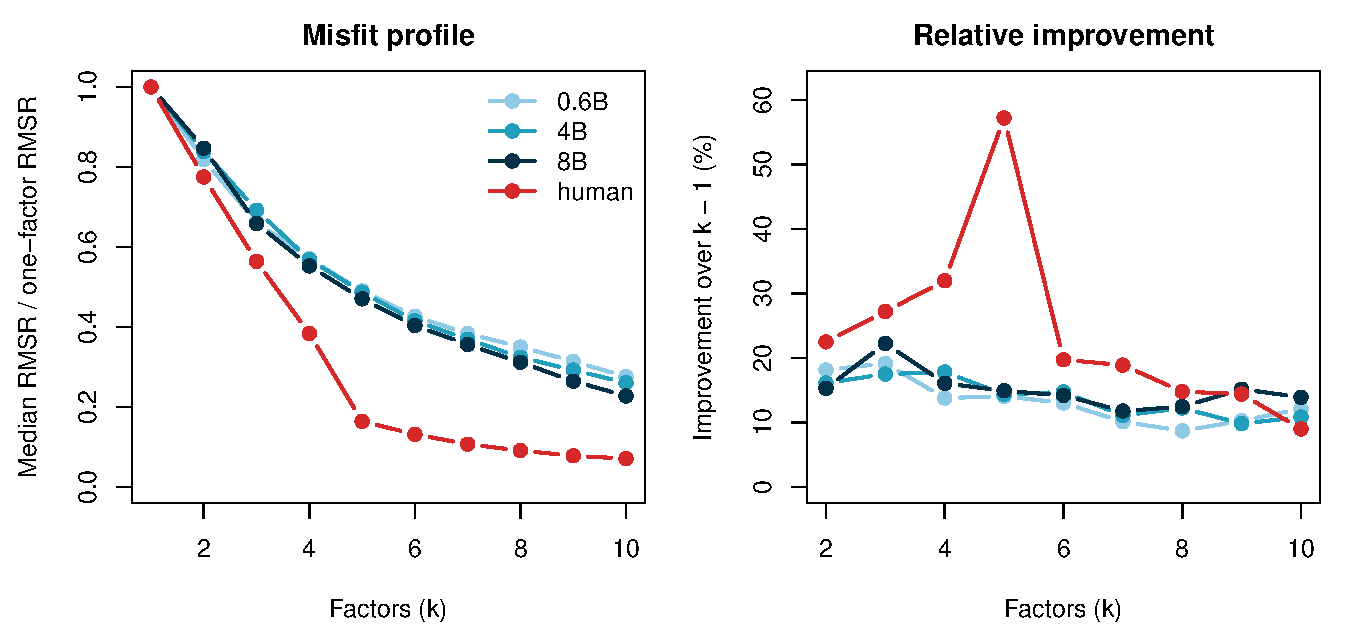
\includegraphics[width=0.95\textwidth]{figures/cd_profiles.pdf}
\captionsetup{justification=raggedright,singlelinecheck=false}
\caption{Comparison-data misfit profiles for the three embedding
similarity matrices (Qwen3-Embedding-0.6B, -4B, -8B) and a keyed human
response subsample ($n = \valCdHumanN$). Left: median root-mean-square
residual (RMSR) between bootstrap-sample eigenvalue profiles and the
observed profile at each candidate factor count, normalized by the
one-factor value. Right: relative improvement over the preceding count.
The human profile shows a sharp elbow at five factors; the embedding
profiles decline smoothly with no elbow at any count.}
\label{fig:cd-profiles}
\end{figure}
